\newpage
\subsection{Долгосрочное планирование продаж}
\label{bp:monthplan}

Долгосрочное (месячное) планирование продаж выполняется в отделе продаж (форма \ref{pic:d2}).
Каждый менеджер создает по своим заказчикам план продаж на будущий месяц по номенклатуре изделий и в количественном выражении. 
План нужен для руководства и для долгосрочного планирования сырья.

% Коммерческий директор контролирует выполнение  плана продаж по отчету ''План продаж'' (рис. \ref{pic:d3}).
% Каждый понедельник все менеджеры формируют в таблице MS Excel план поступления денежных средств для коммерческого директора.





%Менеджеры ведут месячный план продаж в формате MS Excel.
%%План формируется стоимостных (тыс. руб.) показателях.
%Форма плана приведена на рис. \ref{pic:monthplan}.  

%Годовой план продаж разрабатывается коммерческим директором ООО ''ТД «Брянский картон'' и является целевым показателем для других подразделений производства (см. рис. \ref{pic:monthplan}).
%План является необходимым ограничением для менеджеров отдела продаж на год. План формируется в стоимостных (тыс. руб.) показателях.
% 
\begin{figure}
\begin{center}
 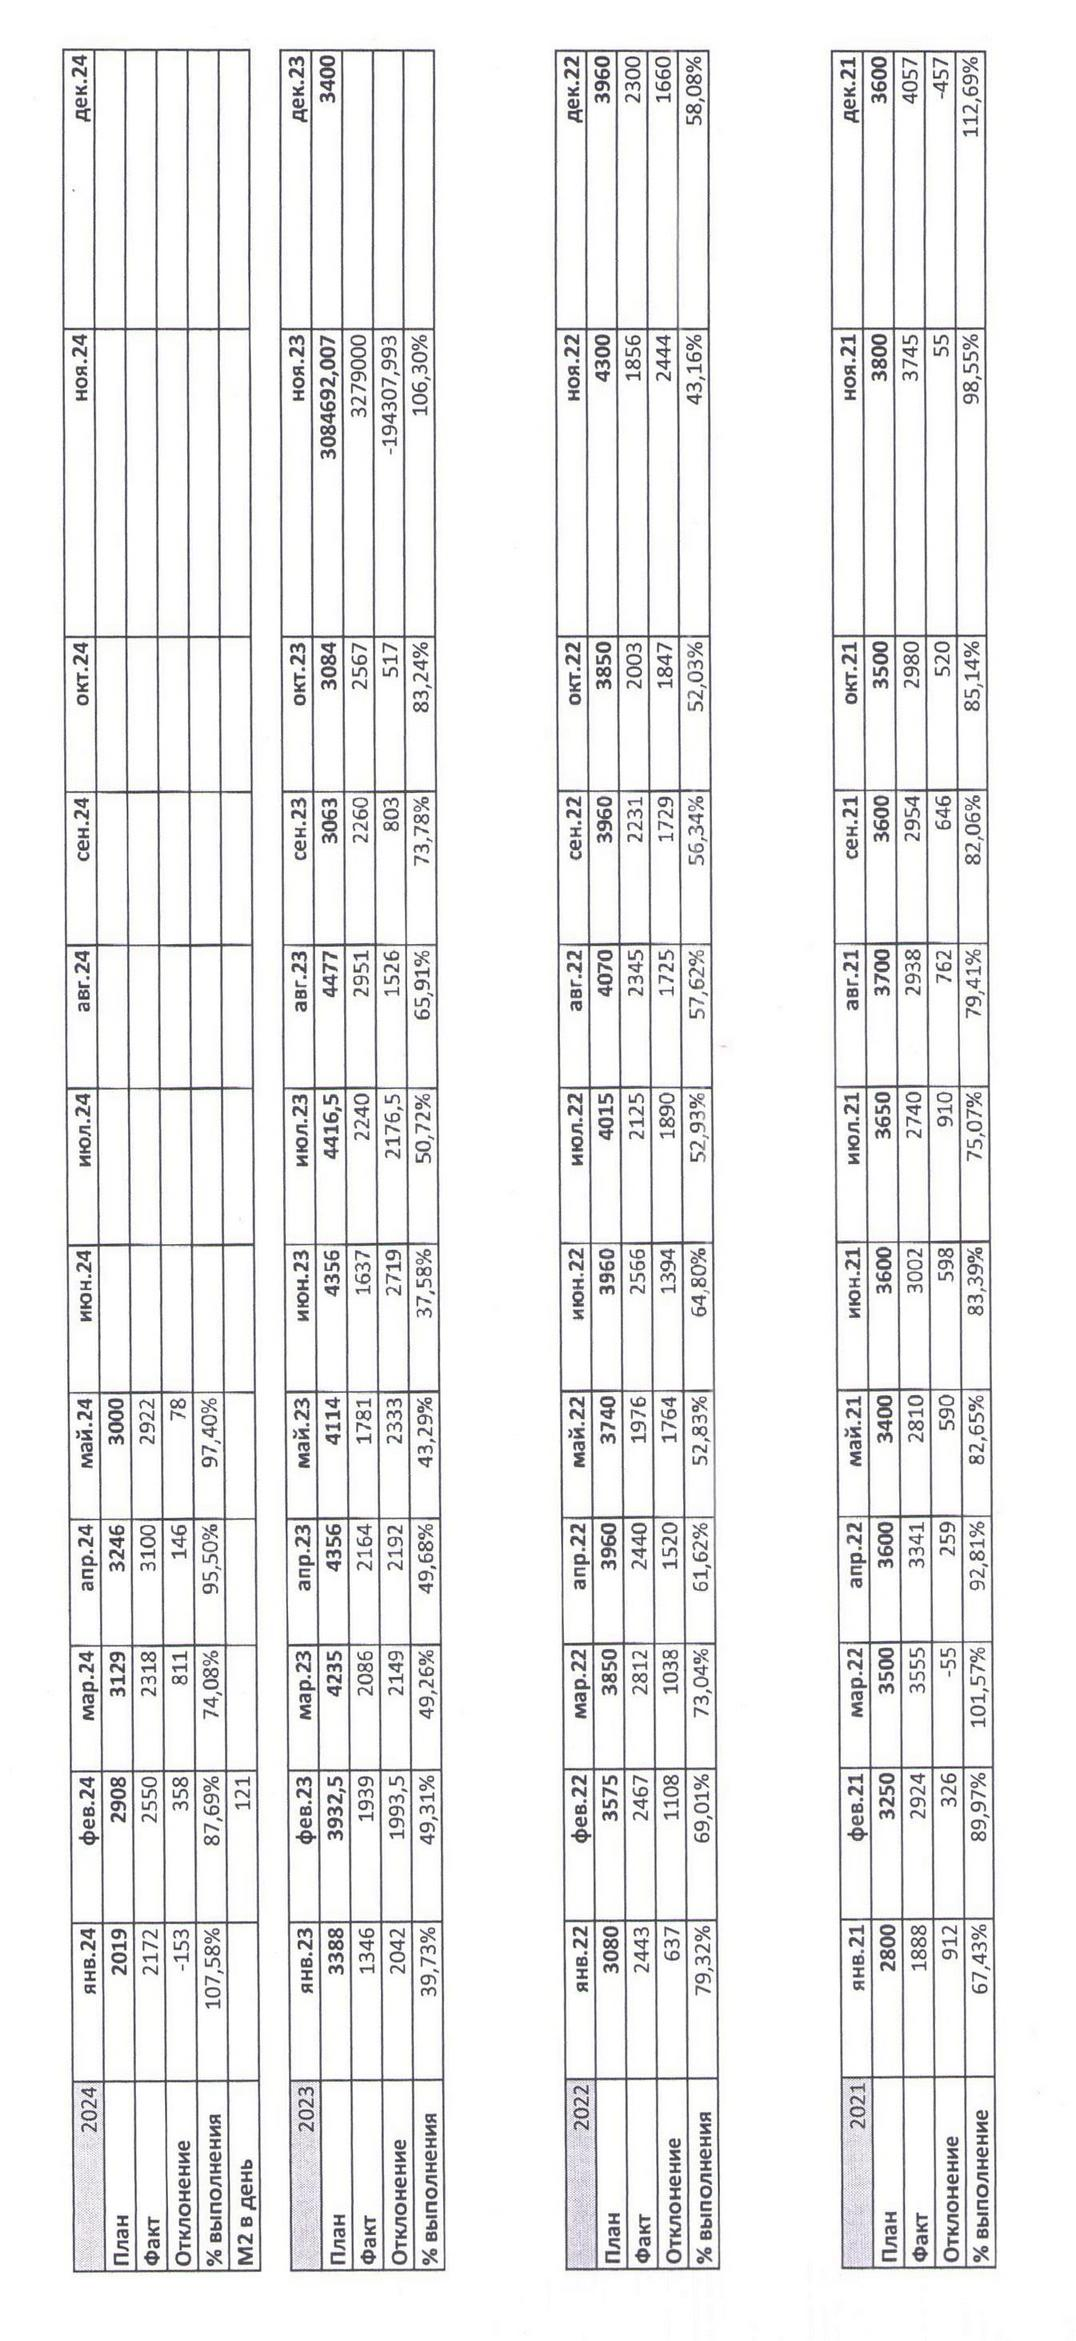
\includegraphics[height=0.8\textheight, width=1.3\textwidth, angle=0, keepaspectratio]{Pics/d02.jpg}
\end{center}
 \caption{Готовой план продаж}
 \label{pic:d2}
\end{figure}
\clearpage


\ifx \notincludehead\undefined
\normalsize
\end{document}
\fi